\documentclass[11pt, a4paper]{article}
\usepackage{pdfpages}
\usepackage{parallel}
\usepackage[T2A]{fontenc}
%\usepackage{ucs}
\usepackage[utf8]{inputenc}
\usepackage[english,russian]{babel}
\usepackage{hyperref}
\usepackage{rotating}
\usepackage[inner=2cm,top=1.8cm,outer=2cm,bottom=2.3cm,nohead]{geometry}
%\usepackage{listings}
\usepackage{graphicx}
\usepackage{wrapfig}
\usepackage{longtable}
\usepackage{indentfirst}
\usepackage{array}
\usepackage{tikzsymbols}
\usepackage{soul}
\usepackage[ruled,vlined]{algorithm2e}
\usepackage{qrcode}
\counterwithout{figure}{section} 

\usepackage{url}
\makeatletter
\g@addto@macro{\UrlBreaks}{\UrlOrds}
\makeatother

\newcolumntype{P}[1]{>{\raggedright\arraybackslash}p{#1}}
\frenchspacing
%\usepackage{fixltx2e} %text sub- and superscripts
\usepackage{icomma} % коскі ў матэматычным рэжыме
%\PreloadUnicodePage{4}

\newcommand{\longpage}{\enlargethispage{\baselineskip}}
\newcommand{\shortpage}{\enlargethispage{-\baselineskip}}

\def\switchlang#1{\expandafter\csname switchlang#1\endcsname}
\def\switchlangbe{
\let\saverefname=\refname%
\def\refname{Літаратура}%
\def\figurename{Іл.}%
}
\def\switchlangru{
\let\saverefname=\refname%
\let\savefigurename=\figurename%
\def\refname{Литература}%
\def\figurename{Рис.}%
}
\def\switchlangen{
\let\saverefname=\refname%
\def\refname{References}%
\def\figurename{Fig.}%
}

\hyphenation{admi-ni-stra-tive}
\hyphenation{ex-pe-ri-ence}
\hyphenation{fle-xi-bi-li-ty}
\hyphenation{Py-thon}
\hyphenation{ma-the-ma-ti-cal}
\hyphenation{re-ported}
\hyphenation{imp-le-menta-tions}
\hyphenation{pro-vides}
\hyphenation{en-gi-neering}
\hyphenation{com-pa-ti-bi-li-ty}
\hyphenation{im-pos-sible}
\hyphenation{desk-top}
\hyphenation{elec-tro-nic}
\hyphenation{com-pa-ny}
\hyphenation{de-ve-lop-ment}
\hyphenation{de-ve-loping}
\hyphenation{de-ve-lop}
\hyphenation{da-ta-ba-se}
\hyphenation{plat-forms}
\hyphenation{or-ga-ni-za-tion}
\hyphenation{pro-gramming}
\hyphenation{in-stru-ments}
\hyphenation{Li-nux}
\hyphenation{sour-ce}
\hyphenation{en-vi-ron-ment}
\hyphenation{Te-le-pathy}
\hyphenation{Li-nux-ov-ka}
\hyphenation{Open-BSD}
\hyphenation{Free-BSD}
\hyphenation{men-ti-on-ed}
\hyphenation{app-li-ca-tion}

\def\progref!#1!{\texttt{#1}}
\renewcommand{\arraystretch}{2} %Іначай формулы ў матрыцы зліпаюцца з лініямі
\usepackage{array}

\def\interview #1 (#2), #3, #4, #5\par{

\section[#1, #3, #4]{#1 -- #3, #4}
\def\qname{LVEE}
\def\aname{#1}
\def\q ##1\par{{\noindent \bf \qname: ##1 }\par}
\def\a{{\noindent \bf \aname: } \def\qname{L}\def\aname{#2}}
}

\def\interview* #1 (#2), #3, #4, #5\par{

\section*{#1\\{\small\rm #3, #4. #5}}
\ifx\ParallelWhichBox\undefined%
    \addcontentsline{toc}{section}{#1, #3, #4}%
\else%
\ifnum\ParallelWhichBox=0%
    \addcontentsline{toc}{section}{#1, #3, #4}%
\fi\fi%

\def\qname{LVEE}
\def\aname{#1}
\def\q ##1\par{{\noindent \bf \qname: ##1 }\par}
\def\a{{\noindent \bf \aname: } \def\qname{L}\def\aname{#2}}
}

\newcommand{\interviewfooter}[1]{
\vskip 1em
\noindent \textit{#1}
}

\AtEndDocument{\vfill\centering \qrcode{https://github.com/fiowro/mouses/blob/main/\jobname.pdf}}

\switchlang{en}
\begin{document}

\title{1987 "--- Sharp KI-OM0002CE01 trackball/mouse combo}
\date{}
\maketitle
\selectlanguage{english}
In 1986, Sharp announced the release of the 16-bit personal computer X68000 for the Japanese market based on the Motorola 68000 processor. The computer went on sale in March 1987. It was positioned as a personal workstation, and immediately attracted attention due to its rich graphics capabilities and audio synthesis (not inferior to the best game consoles of the late 80s), complemented by the unusual design of the system unit in a dual vertical case \cite{museum}. Included with this computer was an unusual convertible mouse (fig. \ref{fig:SharpConvertibleMouse}), which could additionally work as a trackball. Since the device was not intended for separate sale, it received the difficult-to-remember model number KI-OM0002CE01 (when subsequent generations of X68000 computers were released, the mouse model number increased by one, but the mouse itself did not undergo substantial visible changes).

\begin{figure}[h]
    \centering
    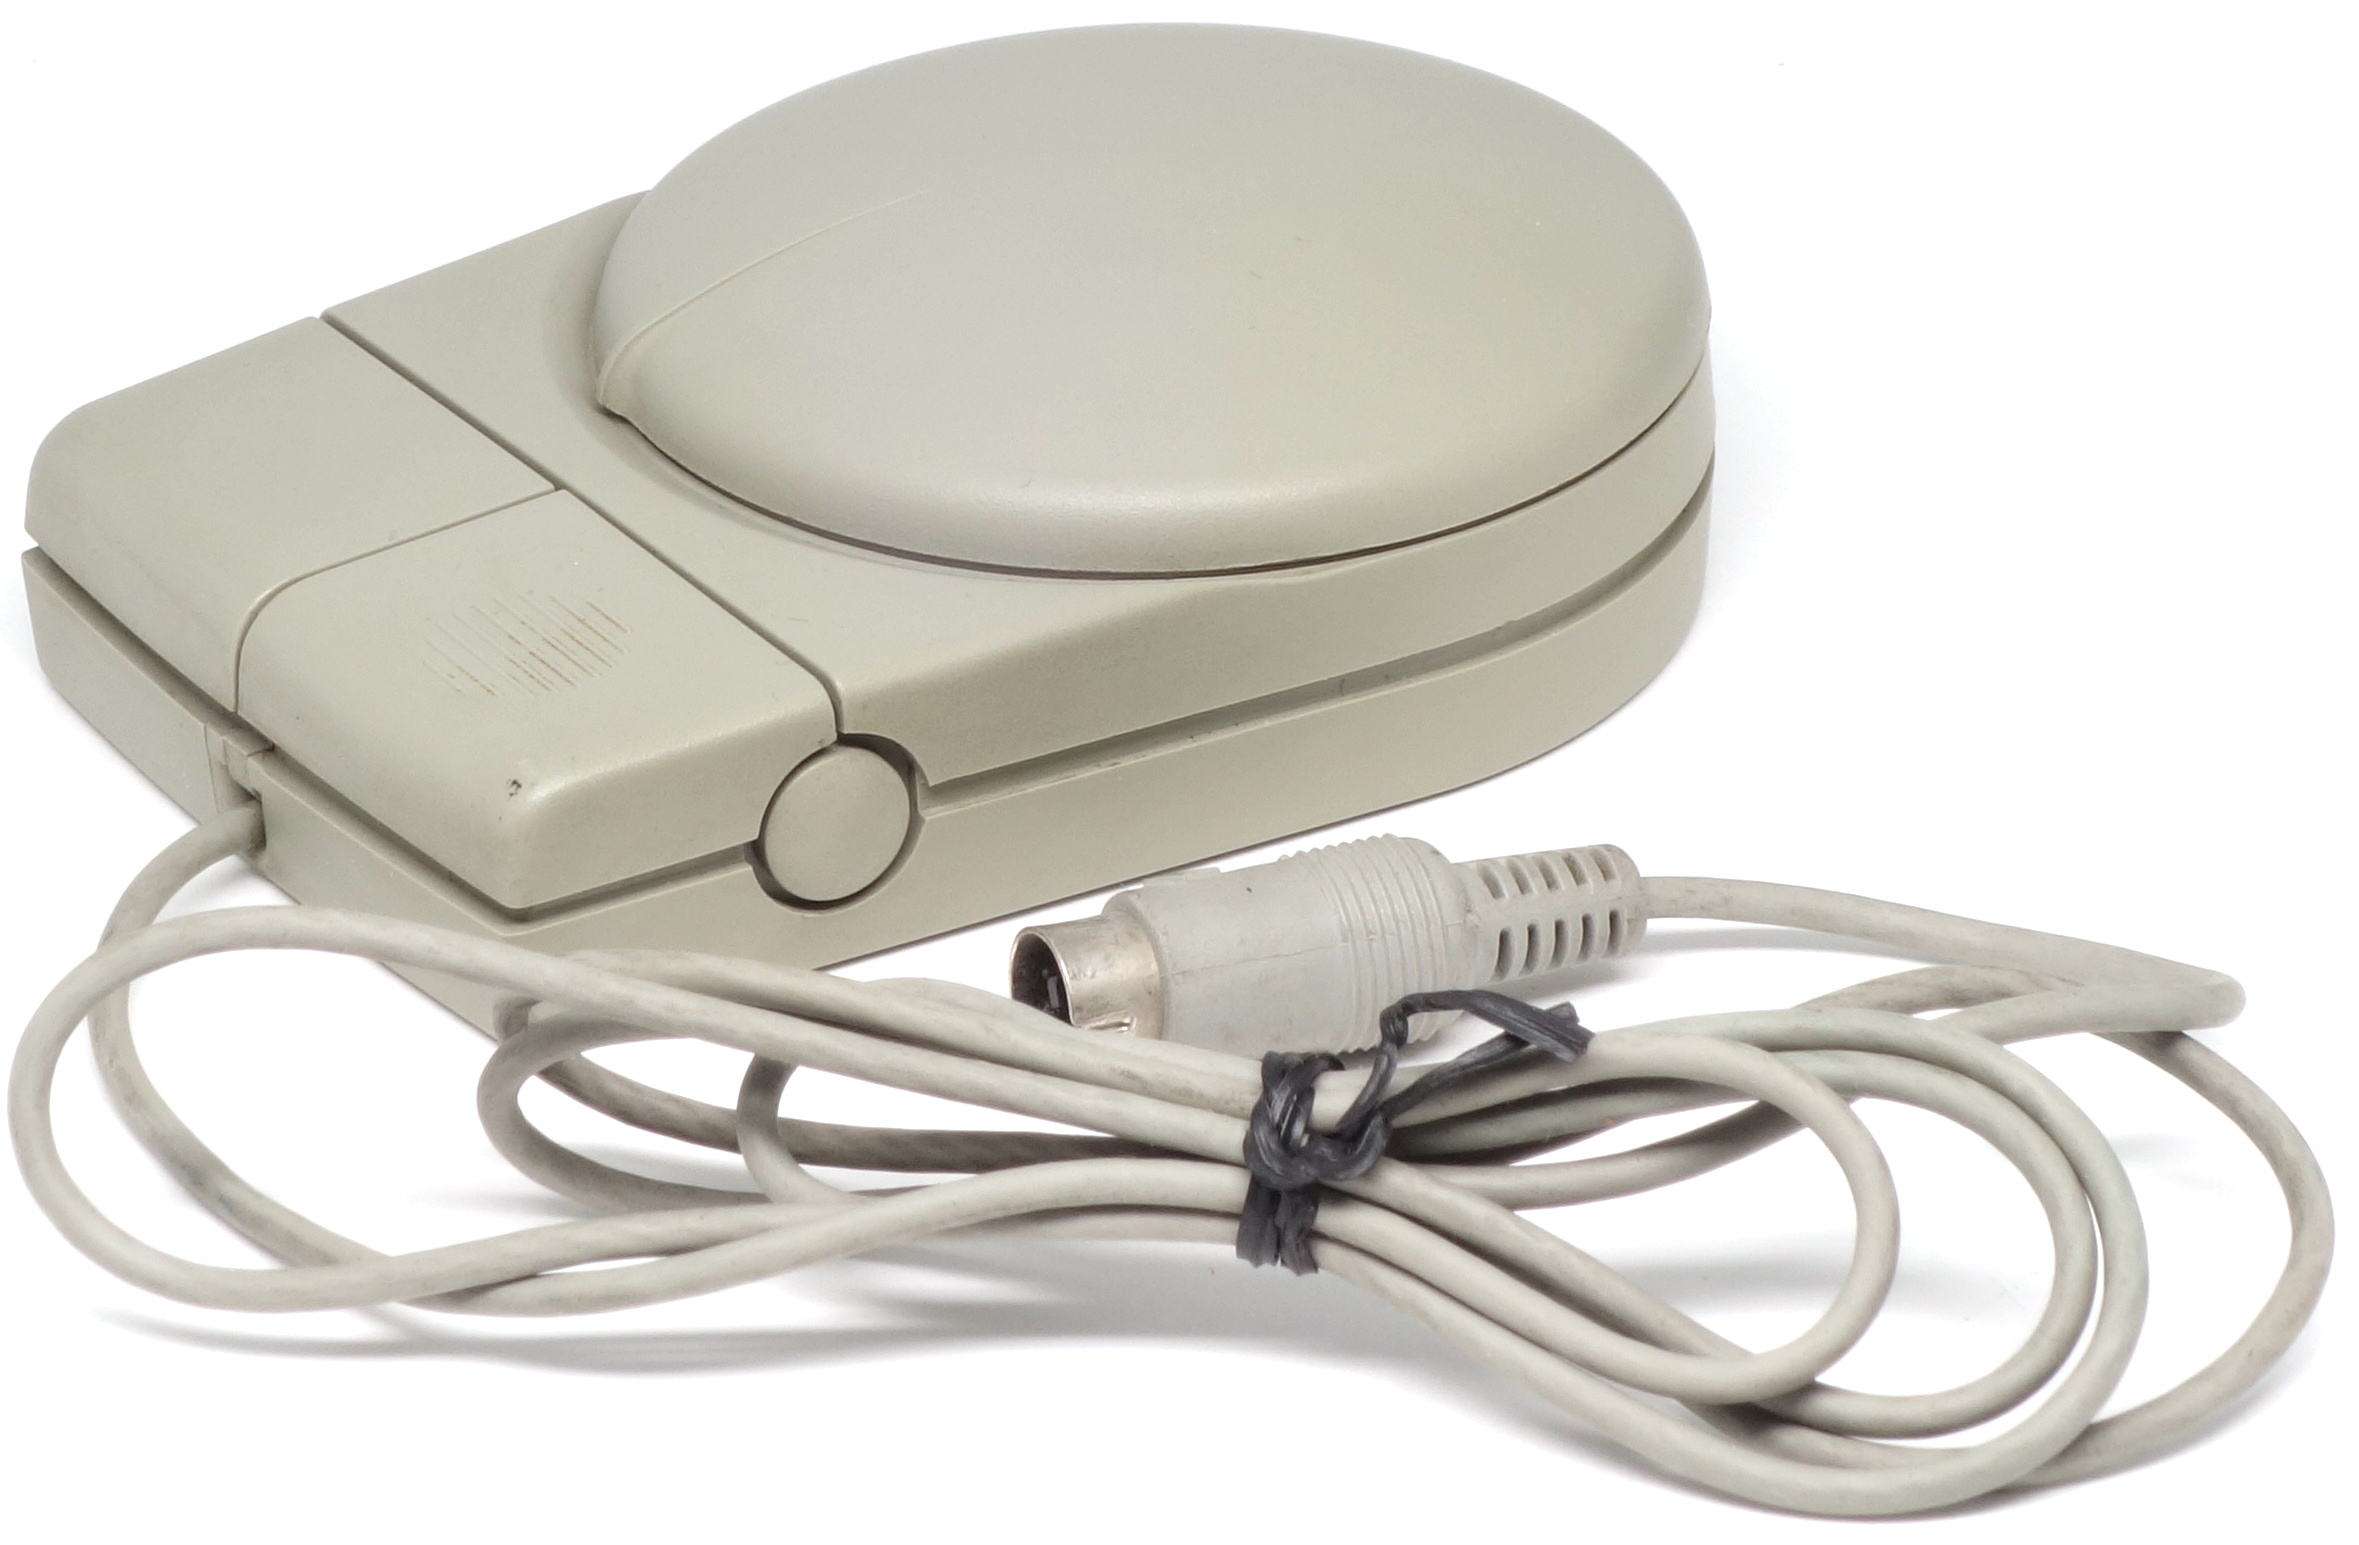
\includegraphics[scale=0.68]{1987_sharp_convertible/picmouse_60}
    \caption{Sharp KI-OM0002CE01, mouse mode}
    \label{fig:SharpConvertibleMouse}
\end{figure}

\begin{figure}[h]
    \centering
    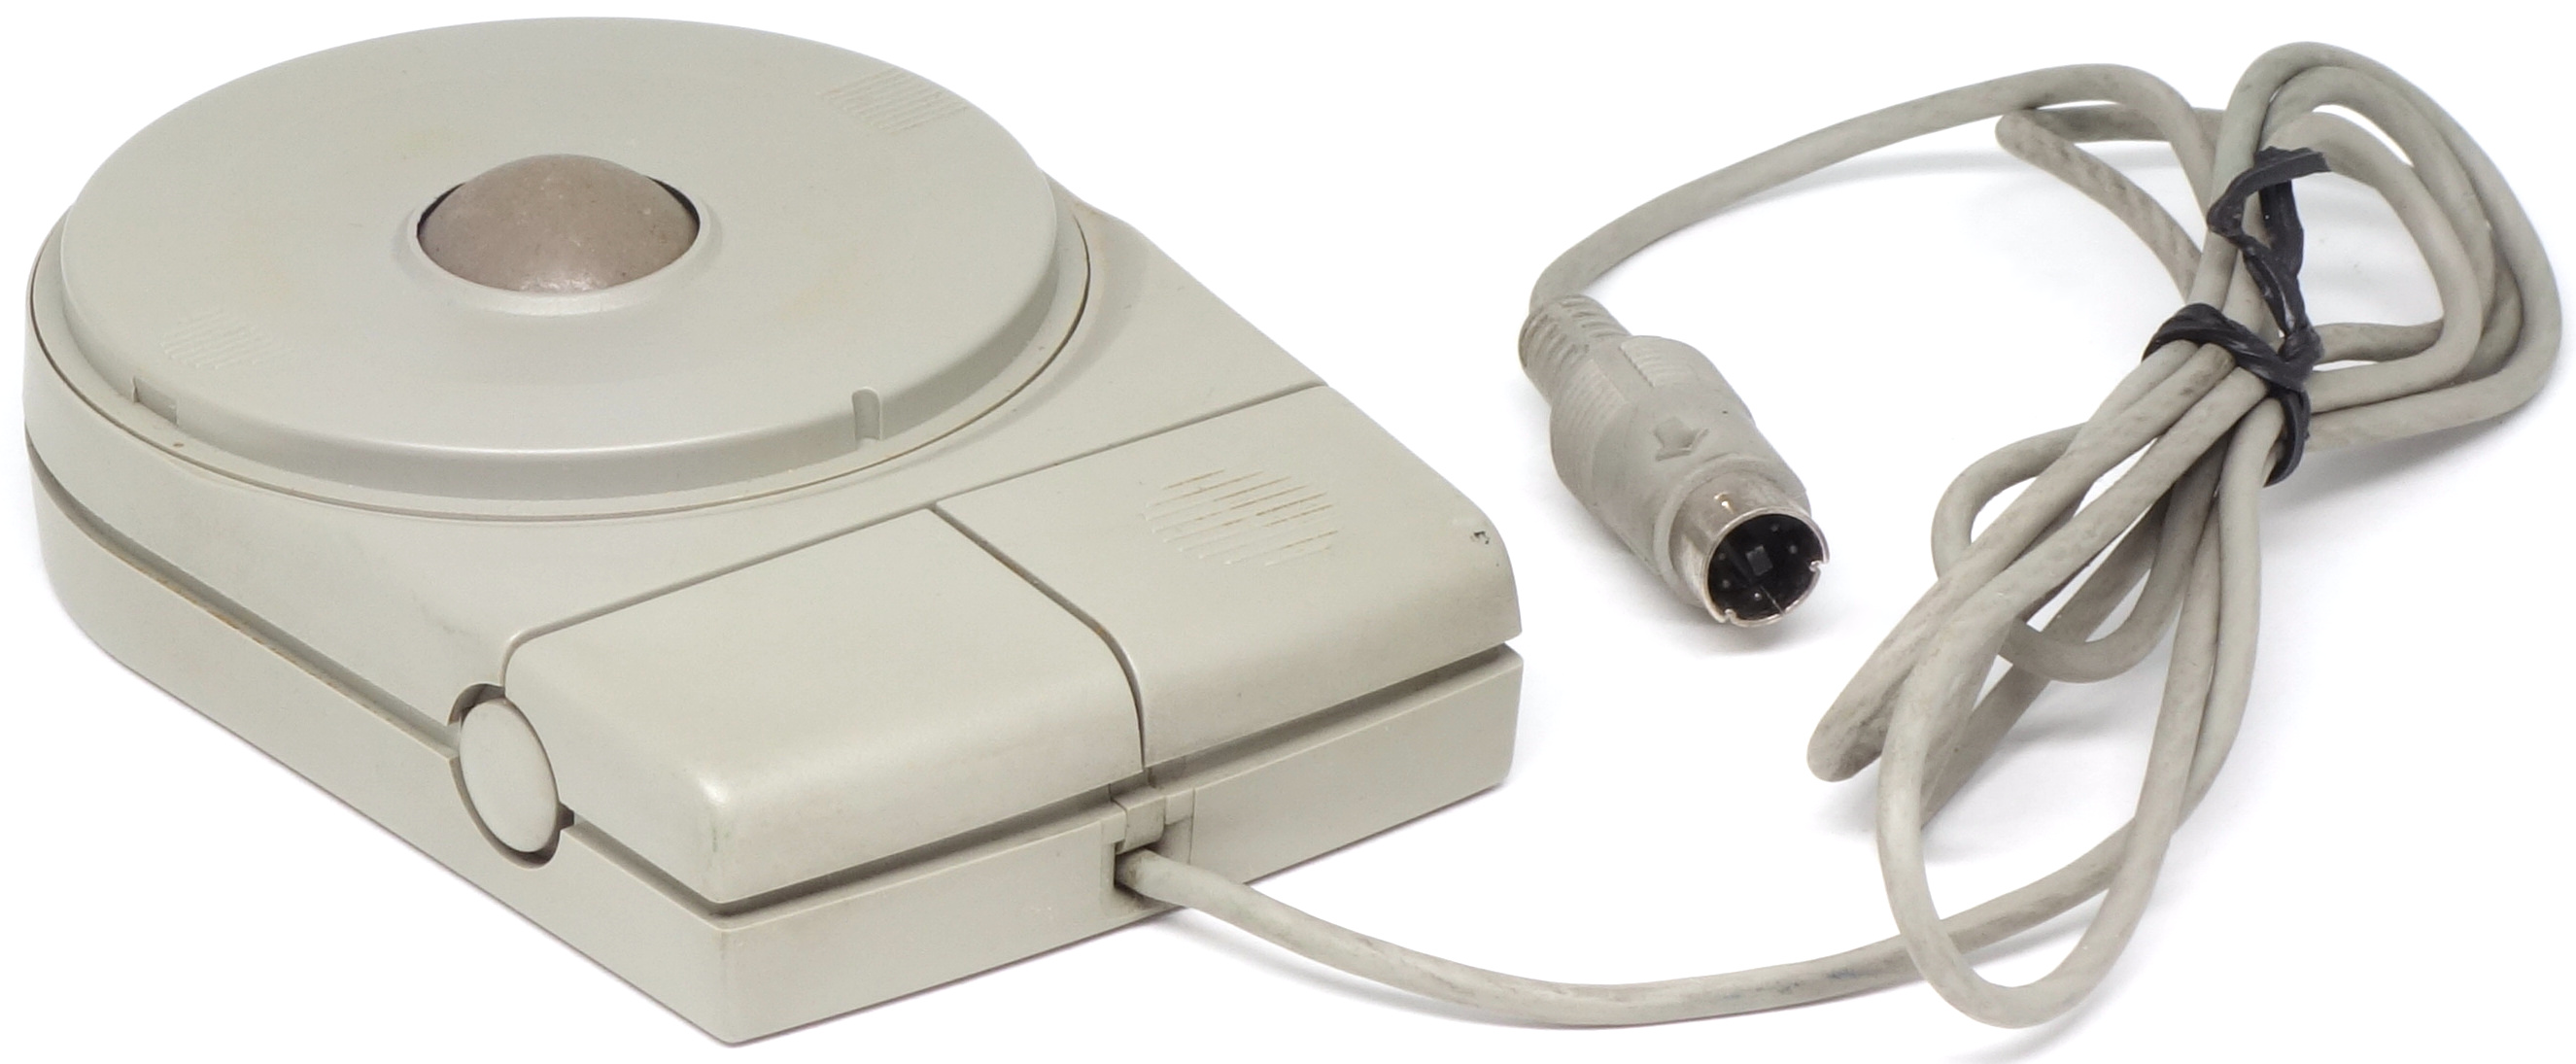
\includegraphics[scale=0.68]{1987_sharp_convertible/picball_60}
    \caption{Sharp KI-OM0002CE01, trackbal mode}
    \label{fig:SharpConvertibleTrackball}
\end{figure}

The design of the mouse shows a commitment to strict geometric shapes, as well as the similarity of the overall shape of the body with the HP 46060A mouse, developed in 1984 by Logitech for Hewlett Packard computers. The mouse body is quite flat, with two large buttons and additional small side buttons on the sides, duplicating the functions of the main buttons \cite{JapaneseVintage}. Two-thirds of the body is occupied by a removable round cover (fig. \ref{fig:SharpConvertibleMouse}), which serves as a support for the palm and at the same time covers the ball. Rotating the cover 90\,$^\circ$ allows you to hook it by the tab and remove it to use the device in trackball mode (Fig. \ref{fig:SharpConvertibleTrackball}). The cover itself is attached to the body with latches and is not rotatable; in fact, the central part of the body rotates - the one that contains the mechanical unit of the device and part of the electronics.

\begin{figure}[h]
    \centering
    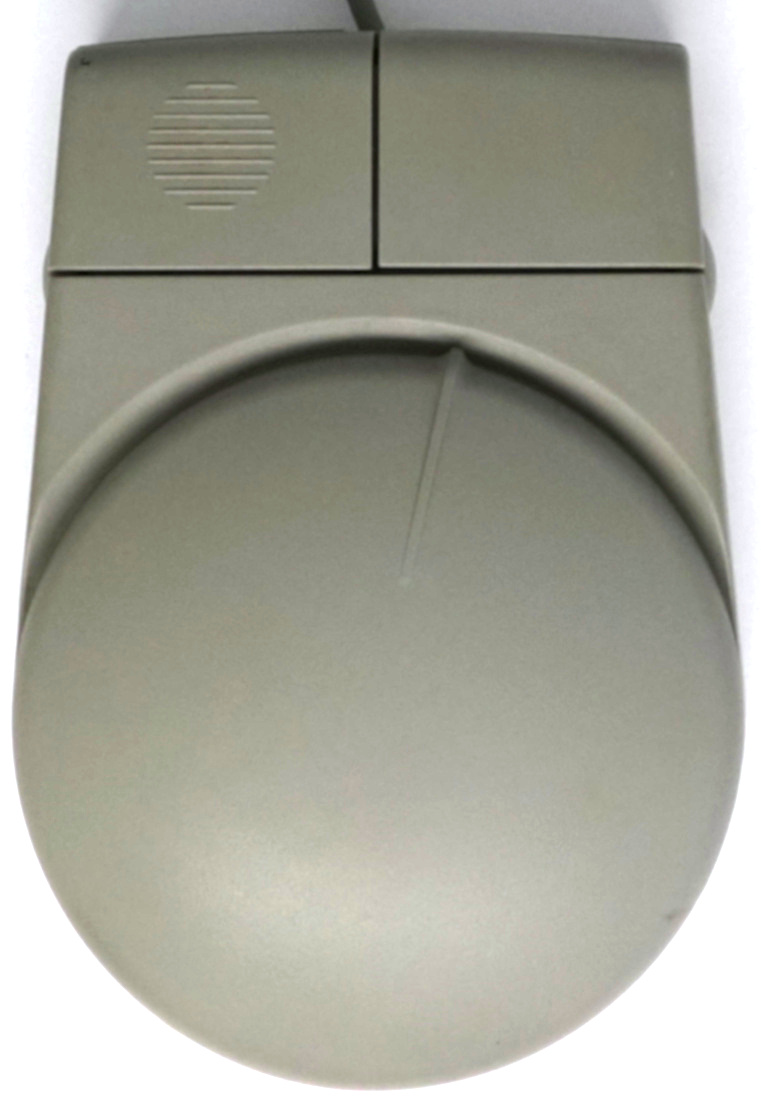
\includegraphics[scale=0.6]{1987_sharp_convertible/top_30.jpg}
    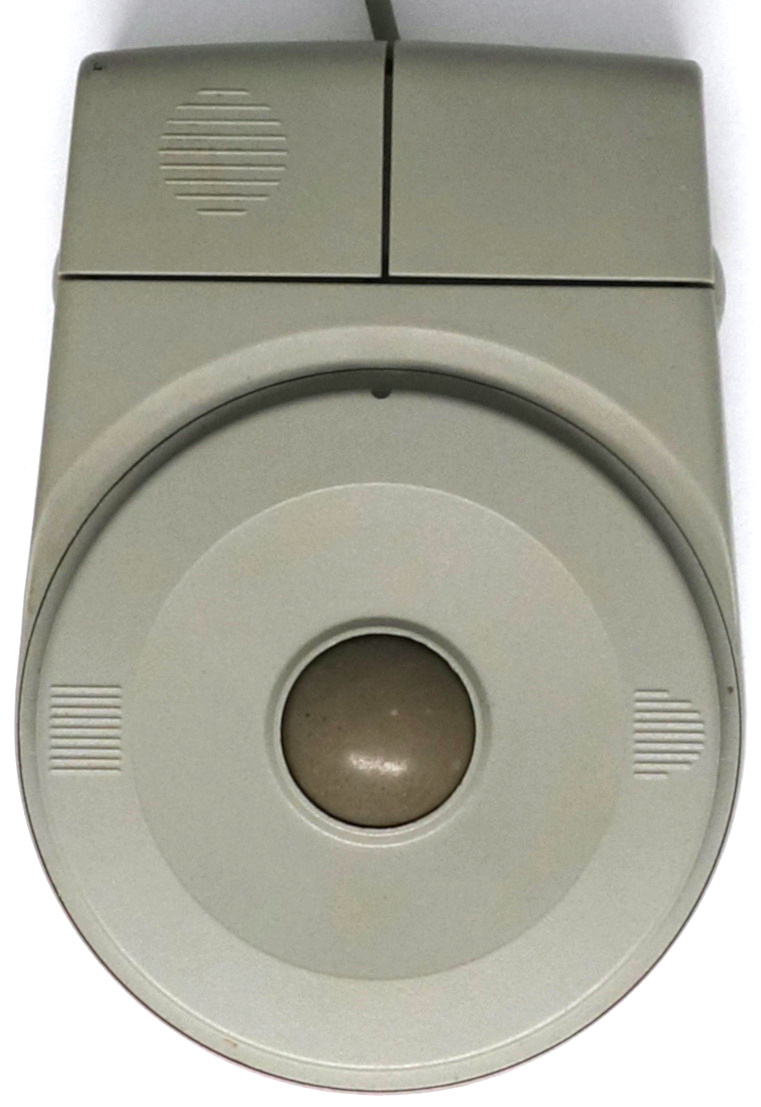
\includegraphics[scale=0.6]{1987_sharp_convertible/topball_30.jpg}
    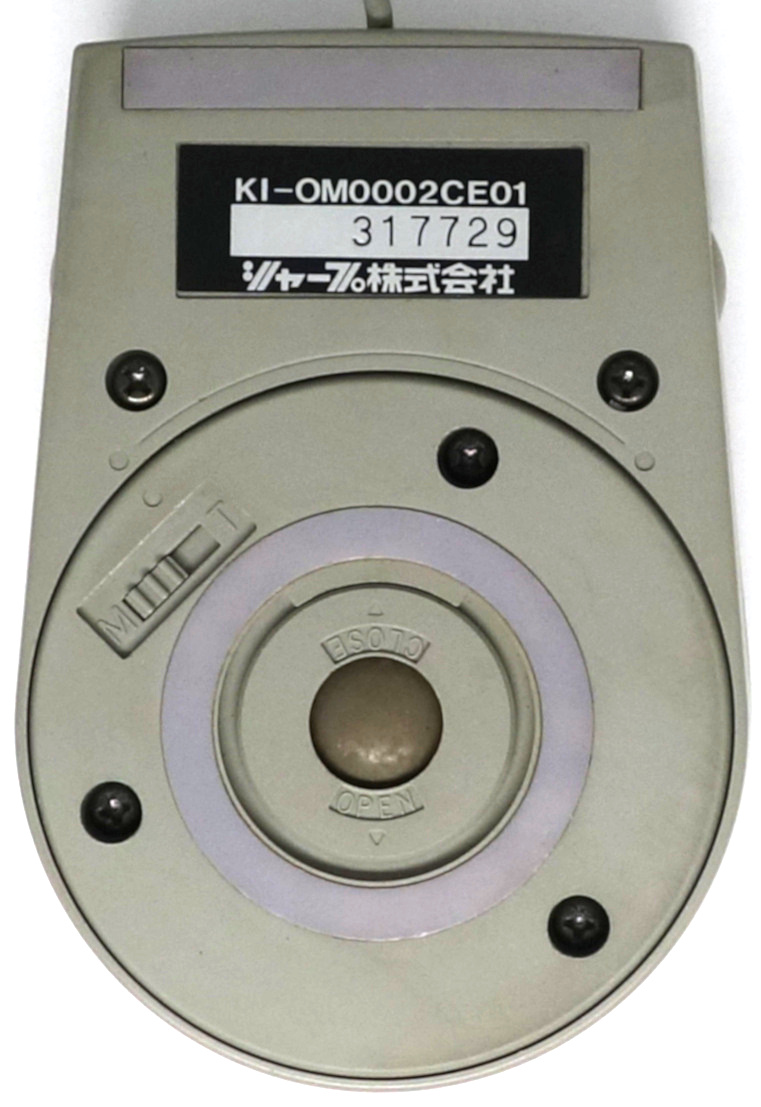
\includegraphics[scale=0.6]{1987_sharp_convertible/bottom_30.jpg}
    \caption{Sharp KI-OM0002CE01: mouse and trackball top views, bottom view}
    \label{fig:SharpConvertibleTopAndBottom}
\end{figure}

To switch to trackball mode, it is not enough to remove the cover: you must also turn the mouse over so that the ball moves to the upper part of the body under the influence of its own weight, and then fix this position of the ball by moving the switch at the bottom of the mouse from  ``M'' to ``T'' position (fig. \ref{fig:SharpConvertibleTopAndBottom}). In addition to the switch, on the bottom side of the case you can see low-friction pads of the standard shape for mice produced by Alps under contract for other companies, as well as a removable ring that allows you to remove the ball for cleaning.

\begin{figure}[h]
    \centering
    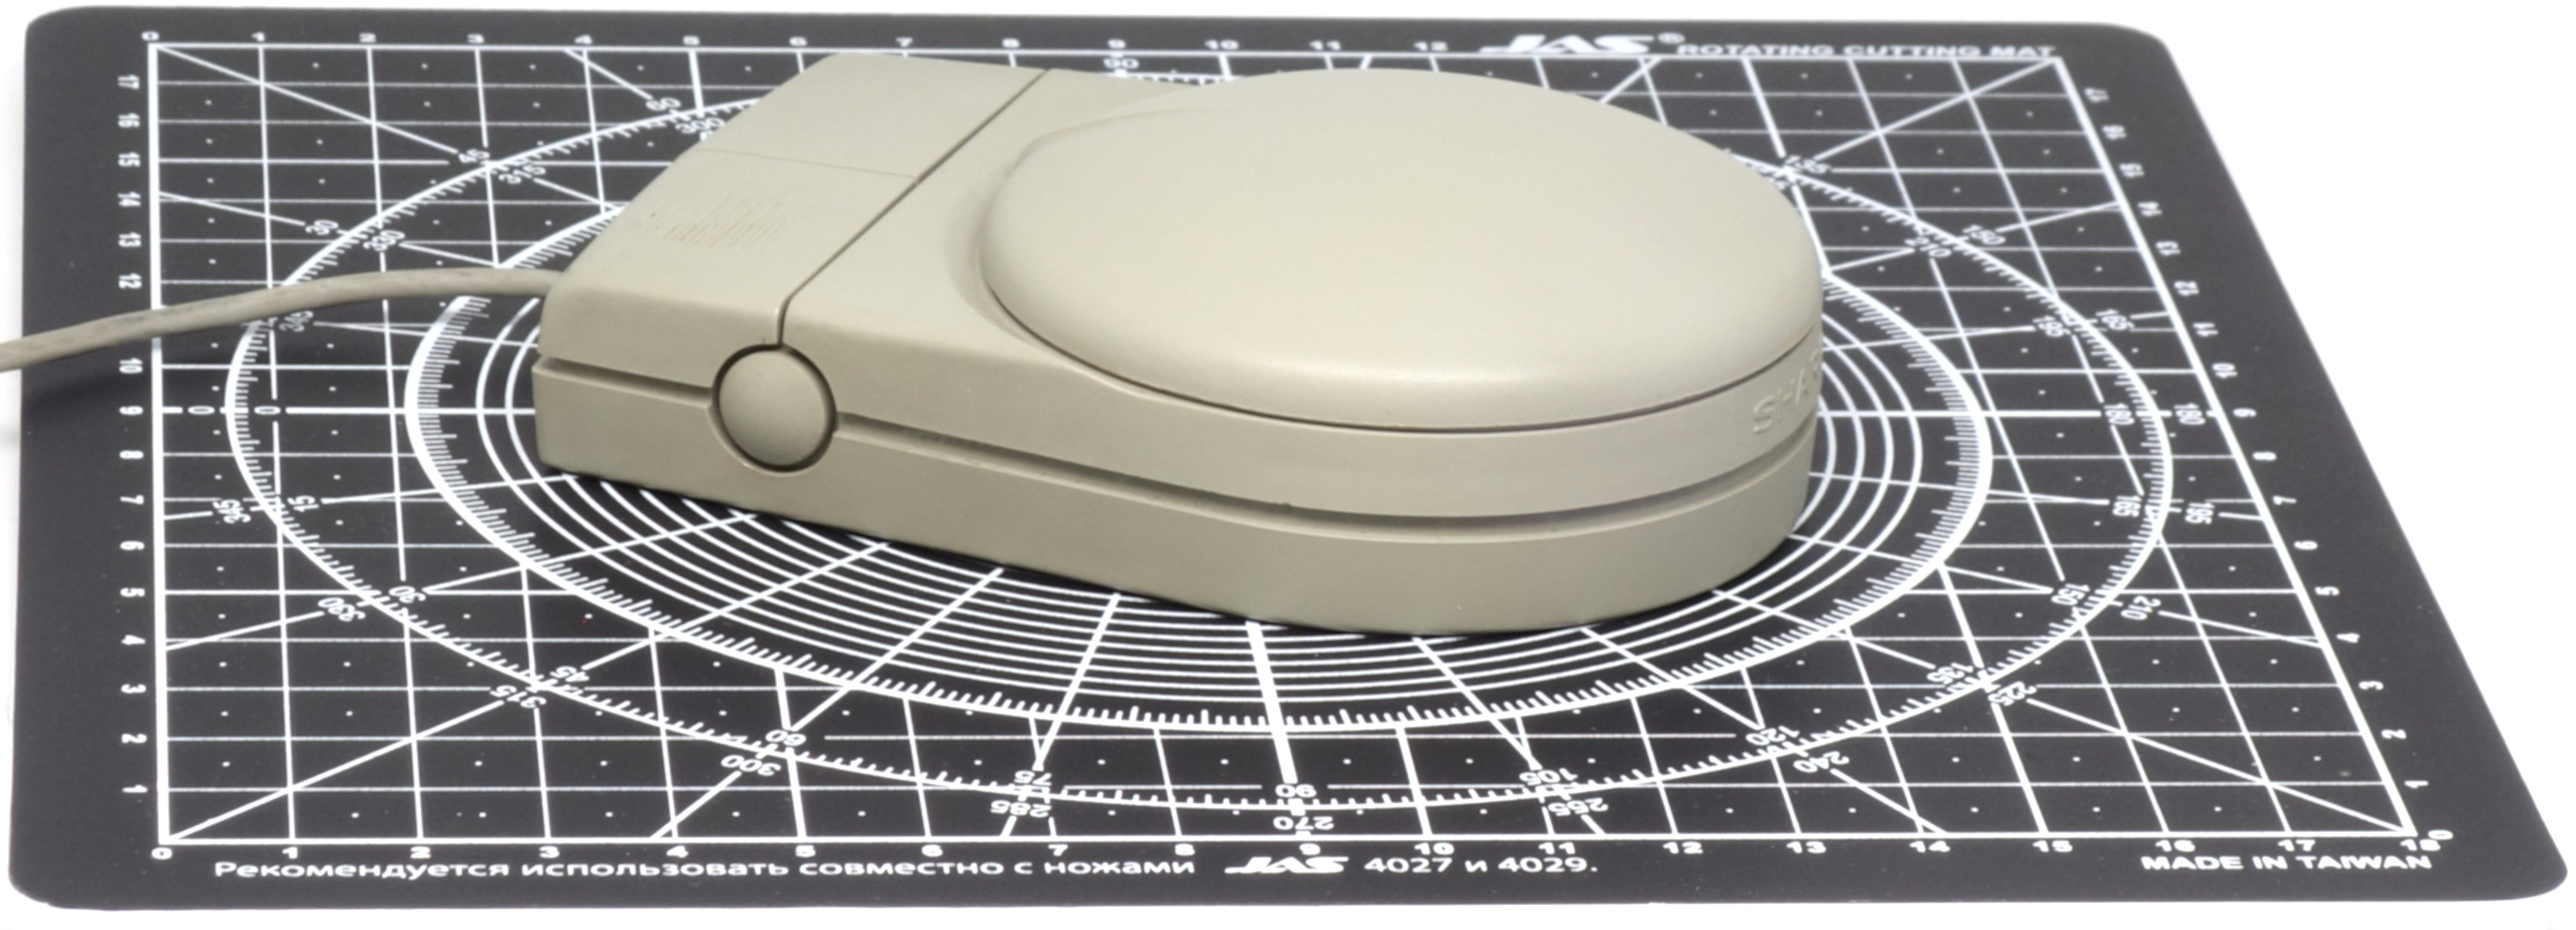
\includegraphics[scale=0.5]{1987_sharp_convertible/size_30.jpg}
    \caption{Sharp KI-OM0002CE01 on a graduated pad with a grid step of 1~cm}
    \label{fig:SharpConvertibleSize}
\end{figure}

Additional elements and the rotating mechanism inside the case did not affect the size of the mouse, which is typical for mice based on standard Alps designs and for the second half of the 80s in general (fig. \ref{fig:SharpConvertibleSize}).

From the point of view of the anatomical structure of the hand, the device has an ergonomic shape, and large buttons are convenient to press with your fingers (fig. \ref{fig:SharpConvertibleHand}). The buttons on the top side of the case, being "fitted" into it, like mice of a later period, have a longer travel when pressed, somewhat similar to the keys of a keyboard, which obviously makes using the mouse a little less convenient. The round pad with relief on the main mouse button indicates the recommended position for your finger \cite{JapaneseClickSense}. A similar relief is applied to two sections of the rotating part of the case under the cover to facilitate its rotation when the cover is removed (fig. \ref{fig:SharpConvertibleTopAndBottom}).

Actually, this rotary unit allows you to work in trackball mode in two ways: classic, when the buttons are located behind the ball (fig. \ref{fig:SharpConvertibleBallHand}), and when the body is rotated 90\,$^\circ$. In this case, the buttons are located to the left of the ball, which obviously implies using the device with two hands in gamepad mode (fig. \ref{fig:SharpConvertiblePadHand}).

\begin{figure}[h]
    \centering
    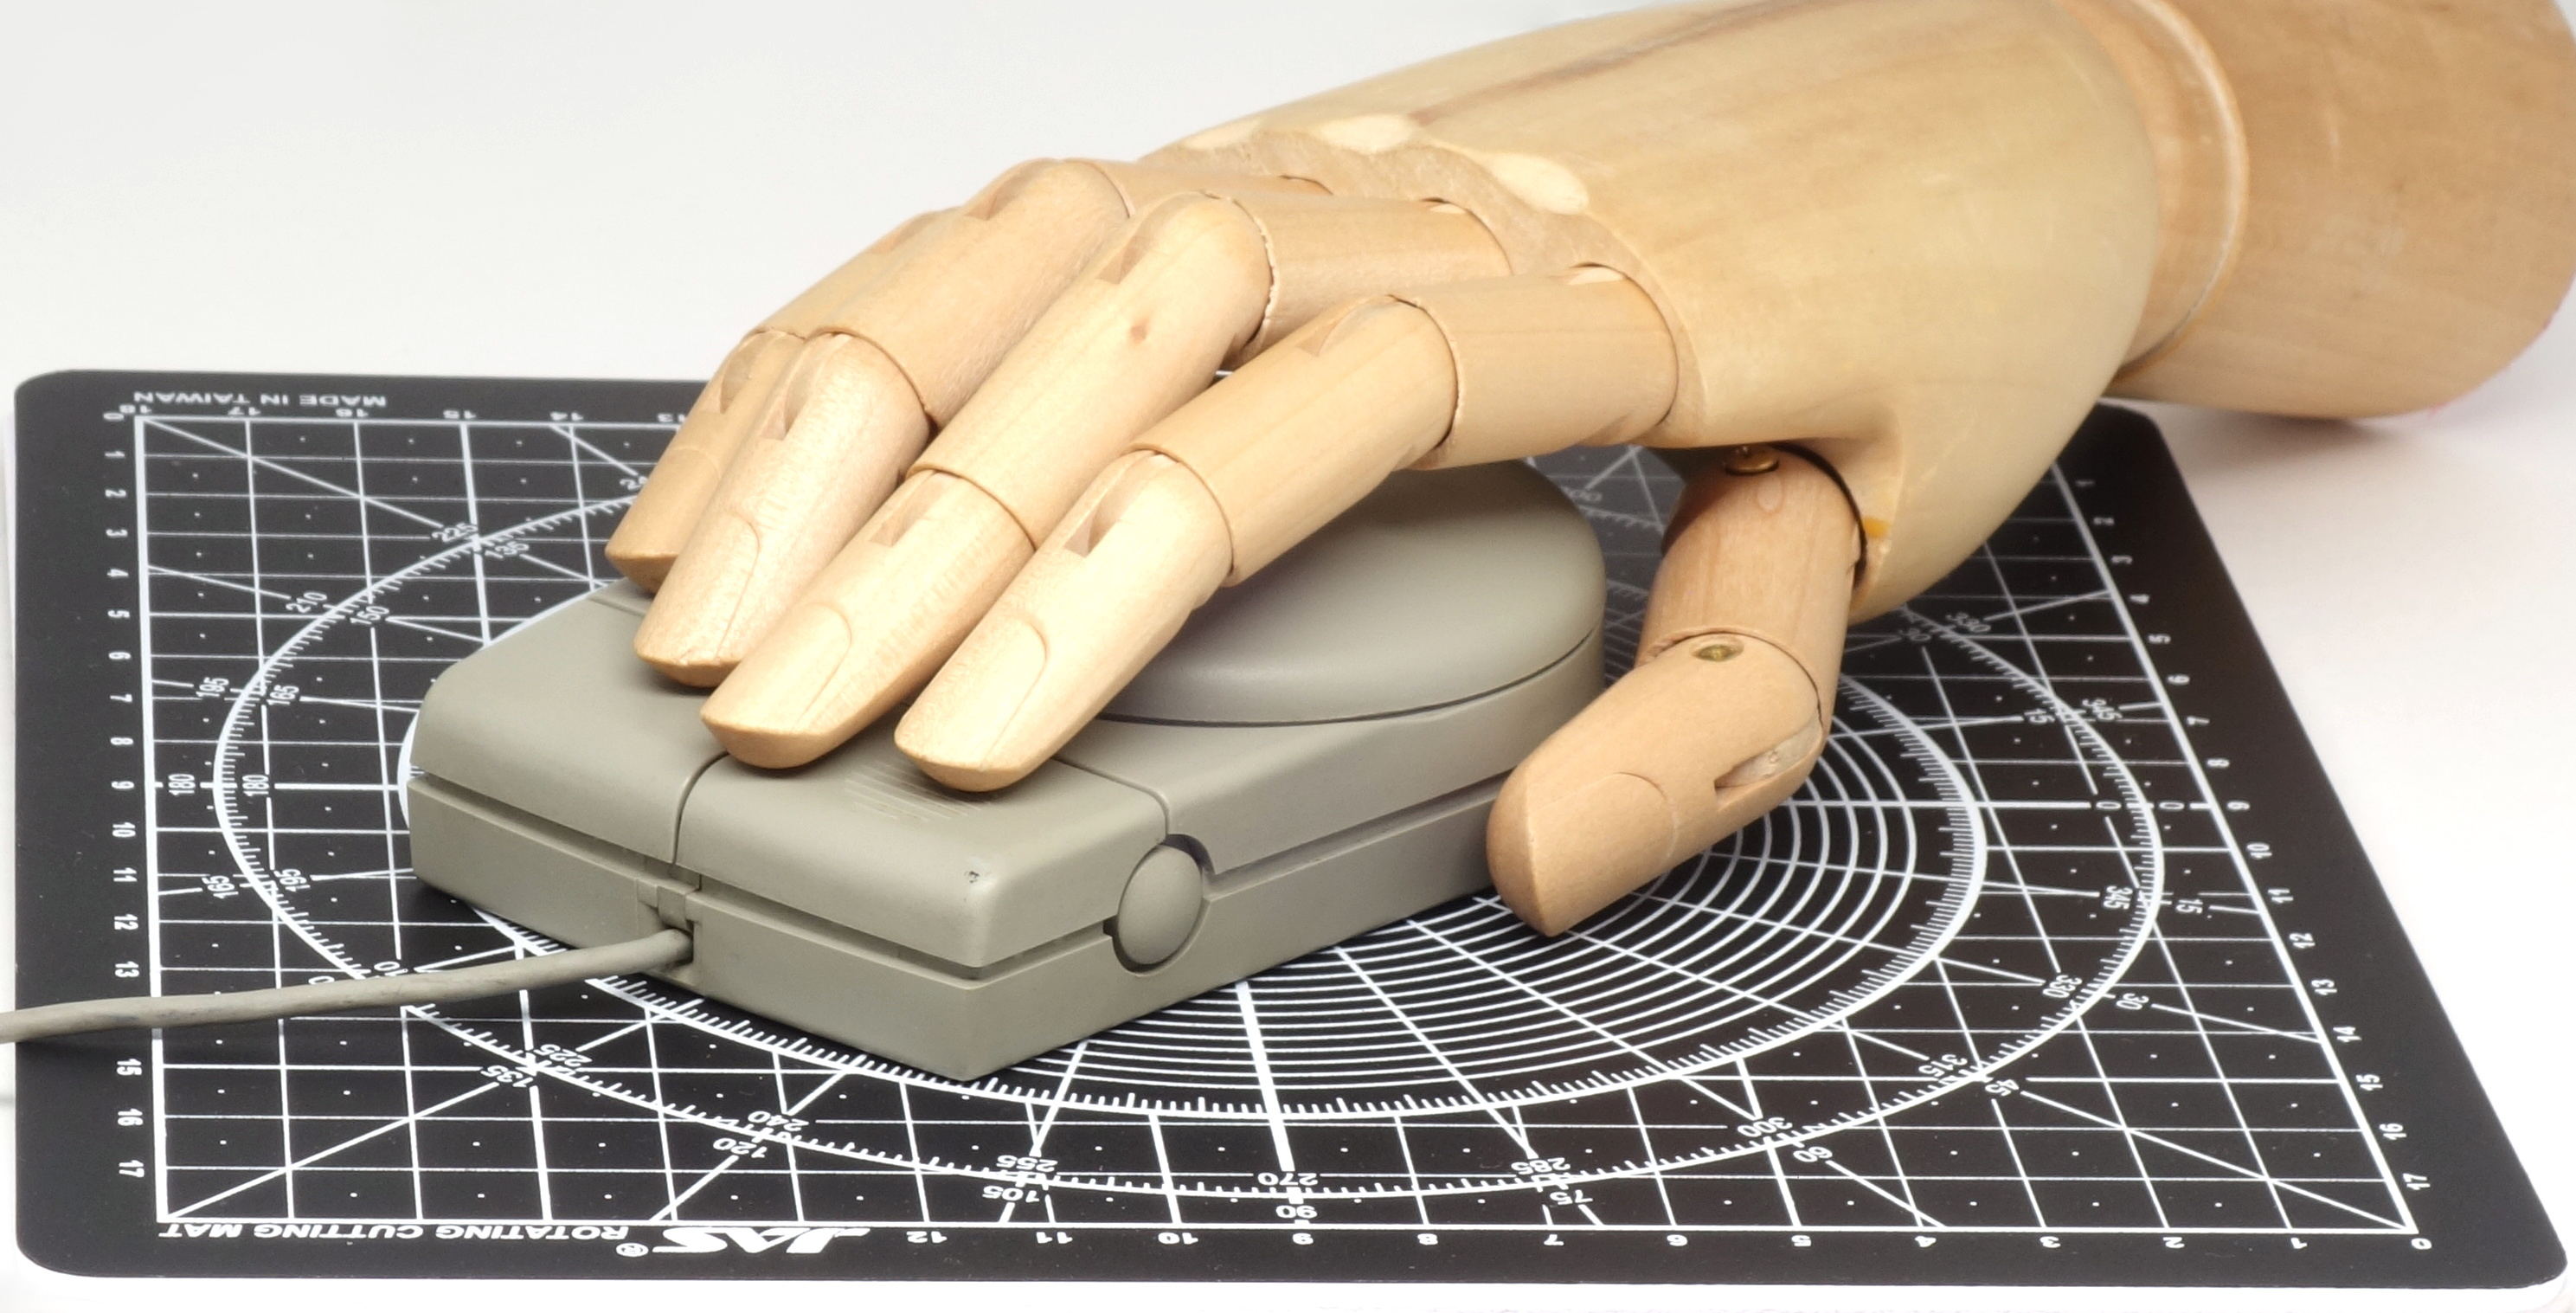
\includegraphics[scale=0.44]{1987_sharp_convertible/handmouse_15.jpg}
    \caption{Sharp KI-OM0002CE01 in mouse mode with a human hand model}
    \label{fig:SharpConvertibleHand}
\end{figure}

\begin{figure}[h]
    \centering
    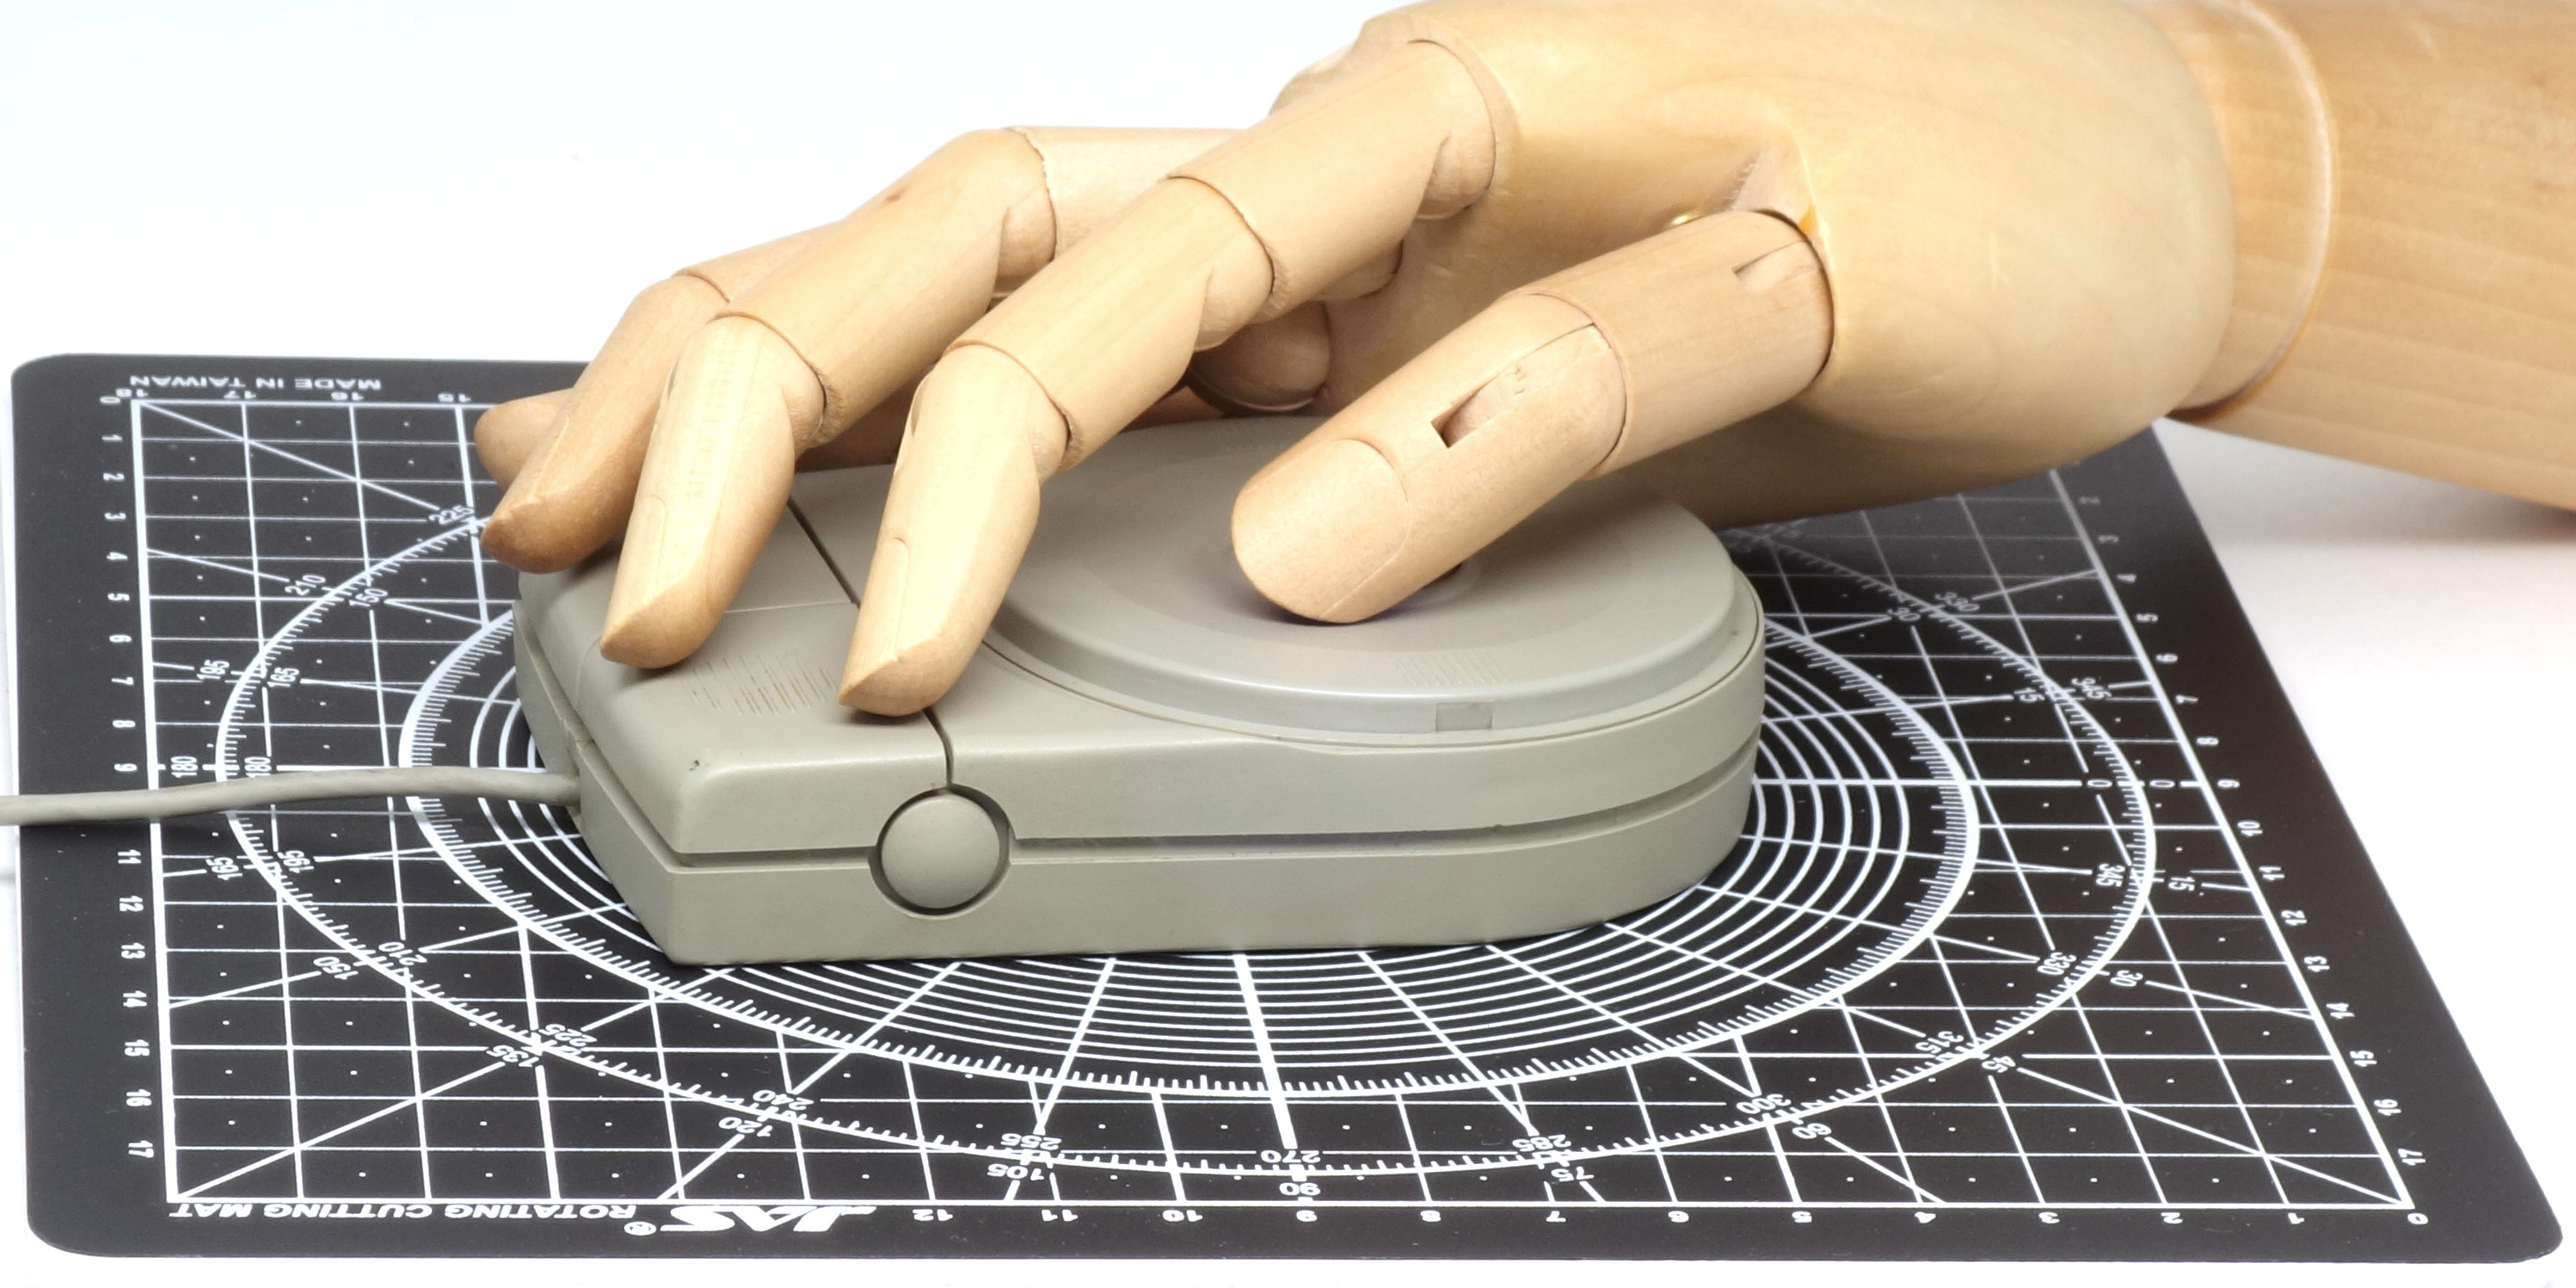
\includegraphics[scale=0.45]{1987_sharp_convertible/handball_30.jpg}
    \caption{Sharp KI-OM0002CE01 in trackball mode with a human hand model}
    \label{fig:SharpConvertibleBallHand}
\end{figure}

\begin{figure}[h]
    \centering
    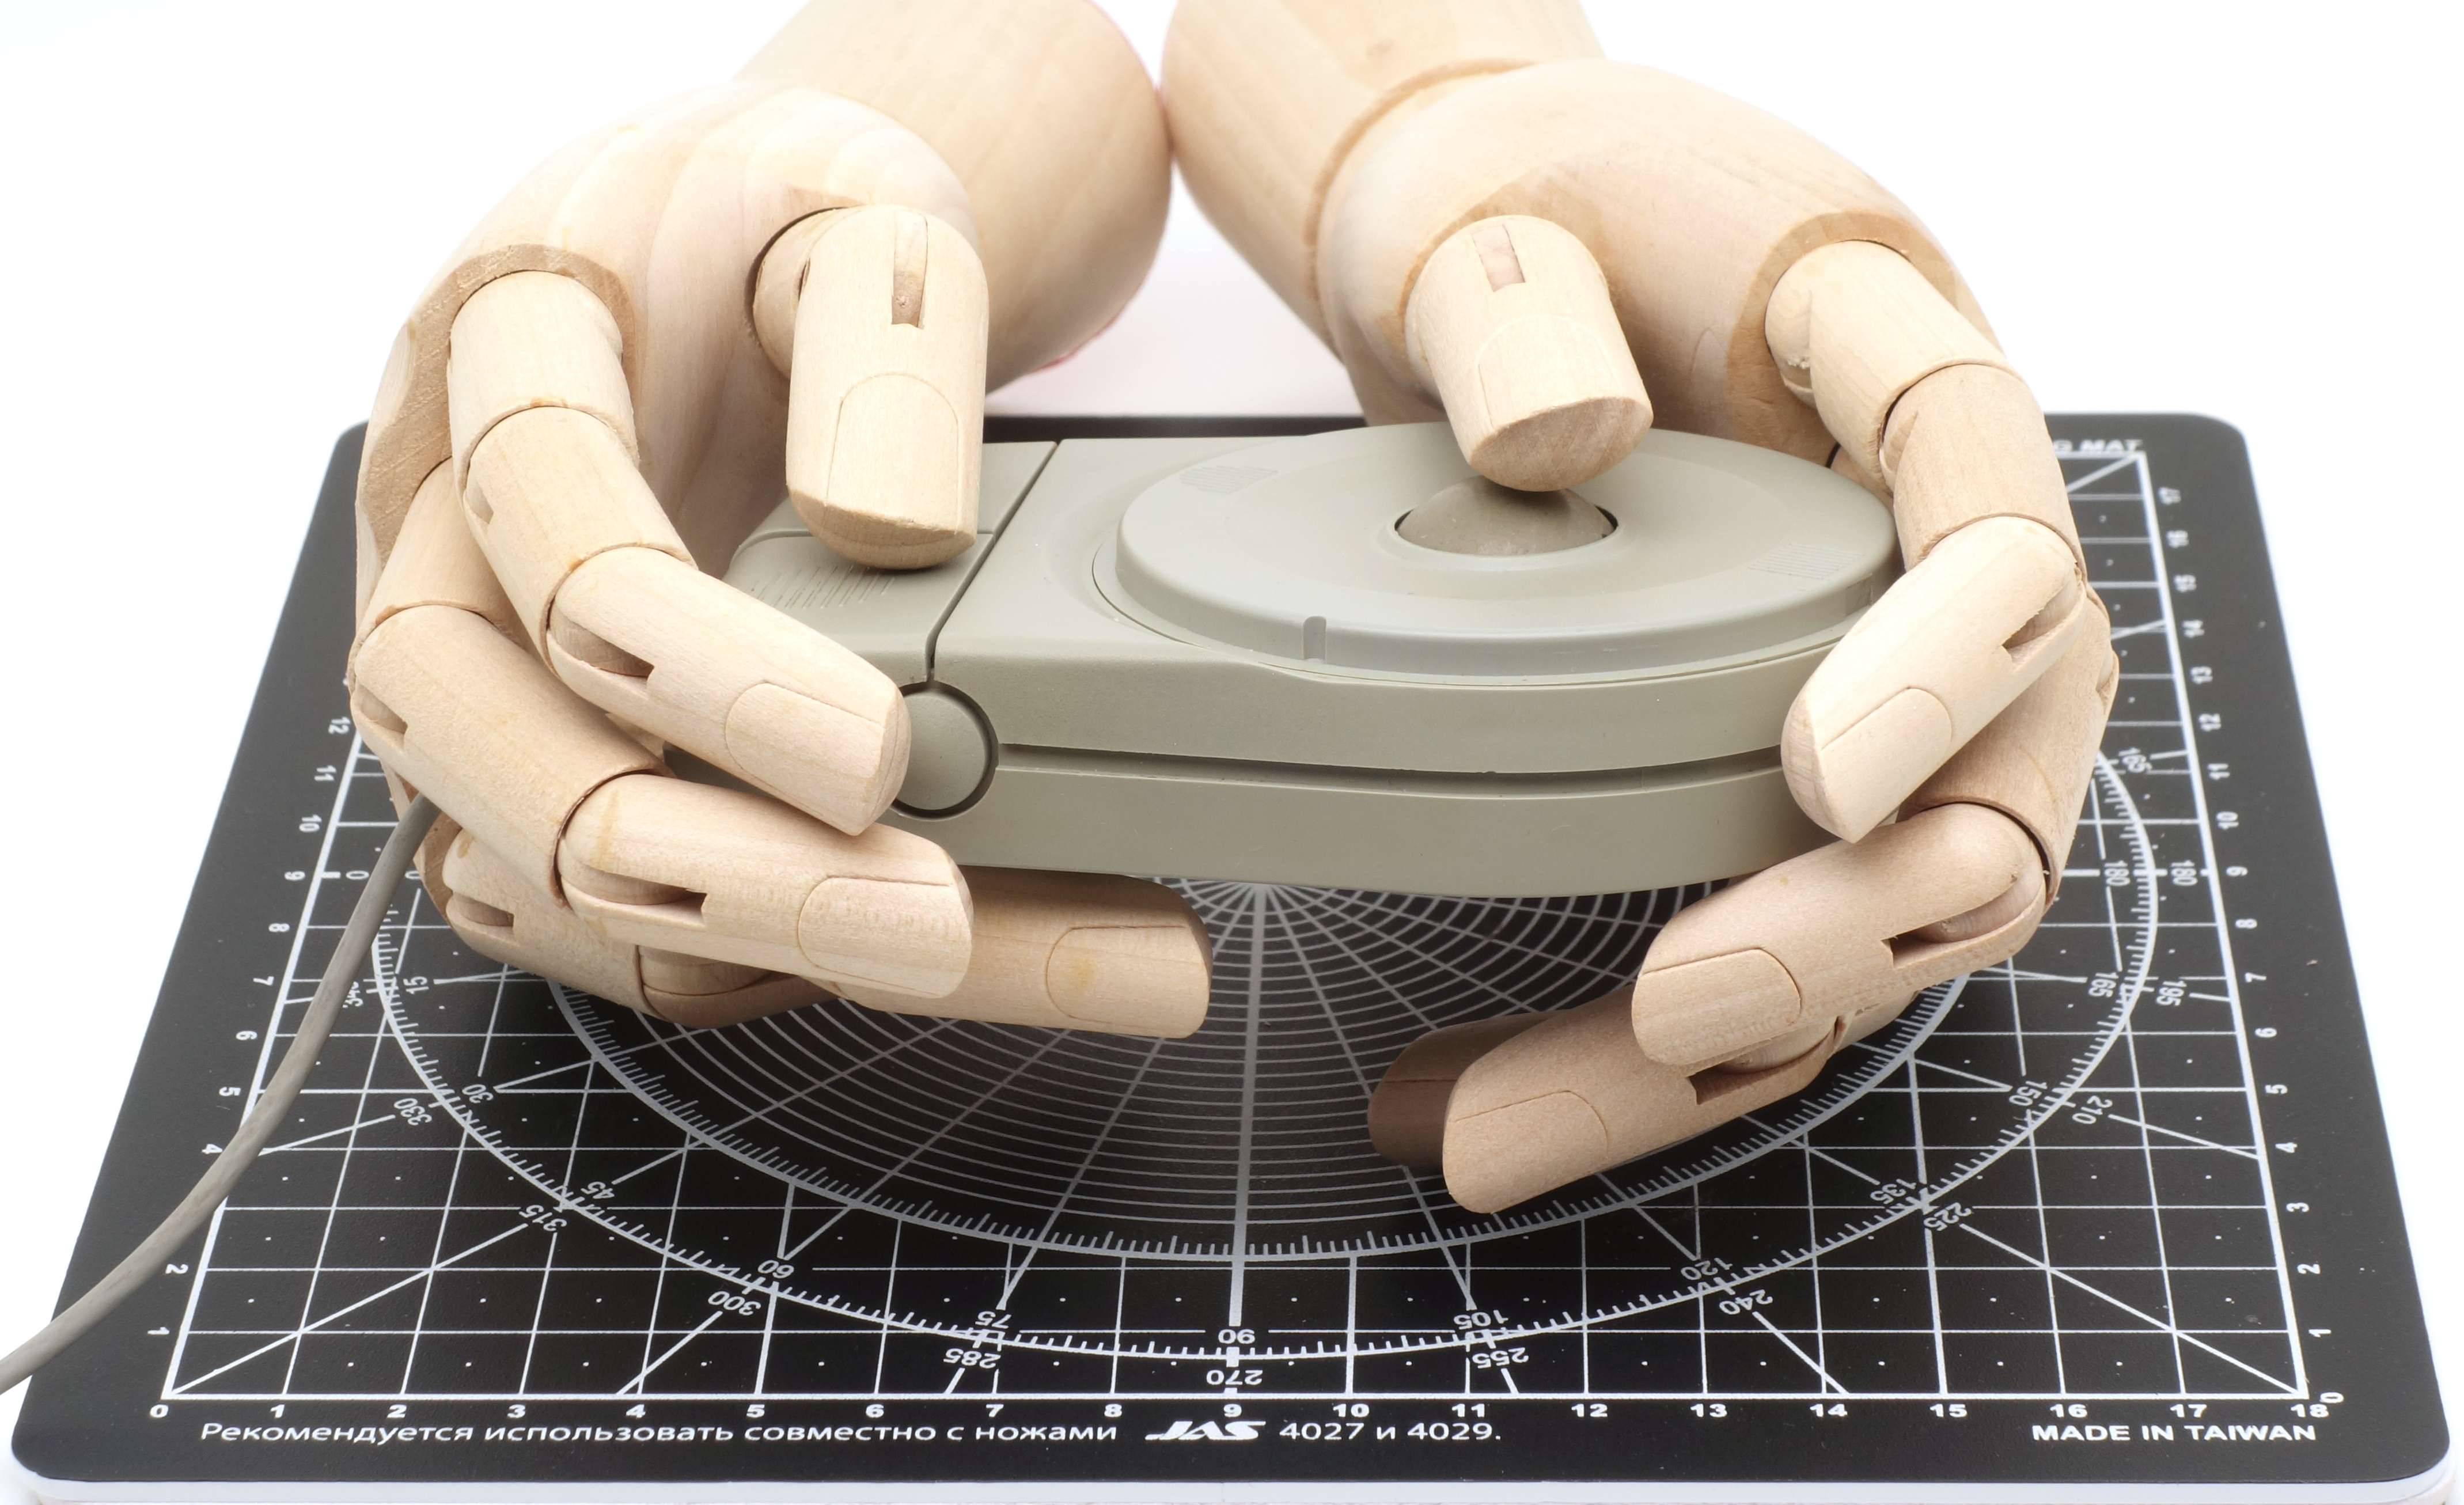
\includegraphics[scale=0.31]{1987_sharp_convertible/handpad_30.jpg}
    \caption{Sharp KI-OM0002CE01 in gamepad mode}
    \label{fig:SharpConvertiblePadHand}
\end{figure}


Trackball internals are shown on figure (\ref{fig:SharpConvertibleInside}).

\begin{figure}[h]
    \centering
    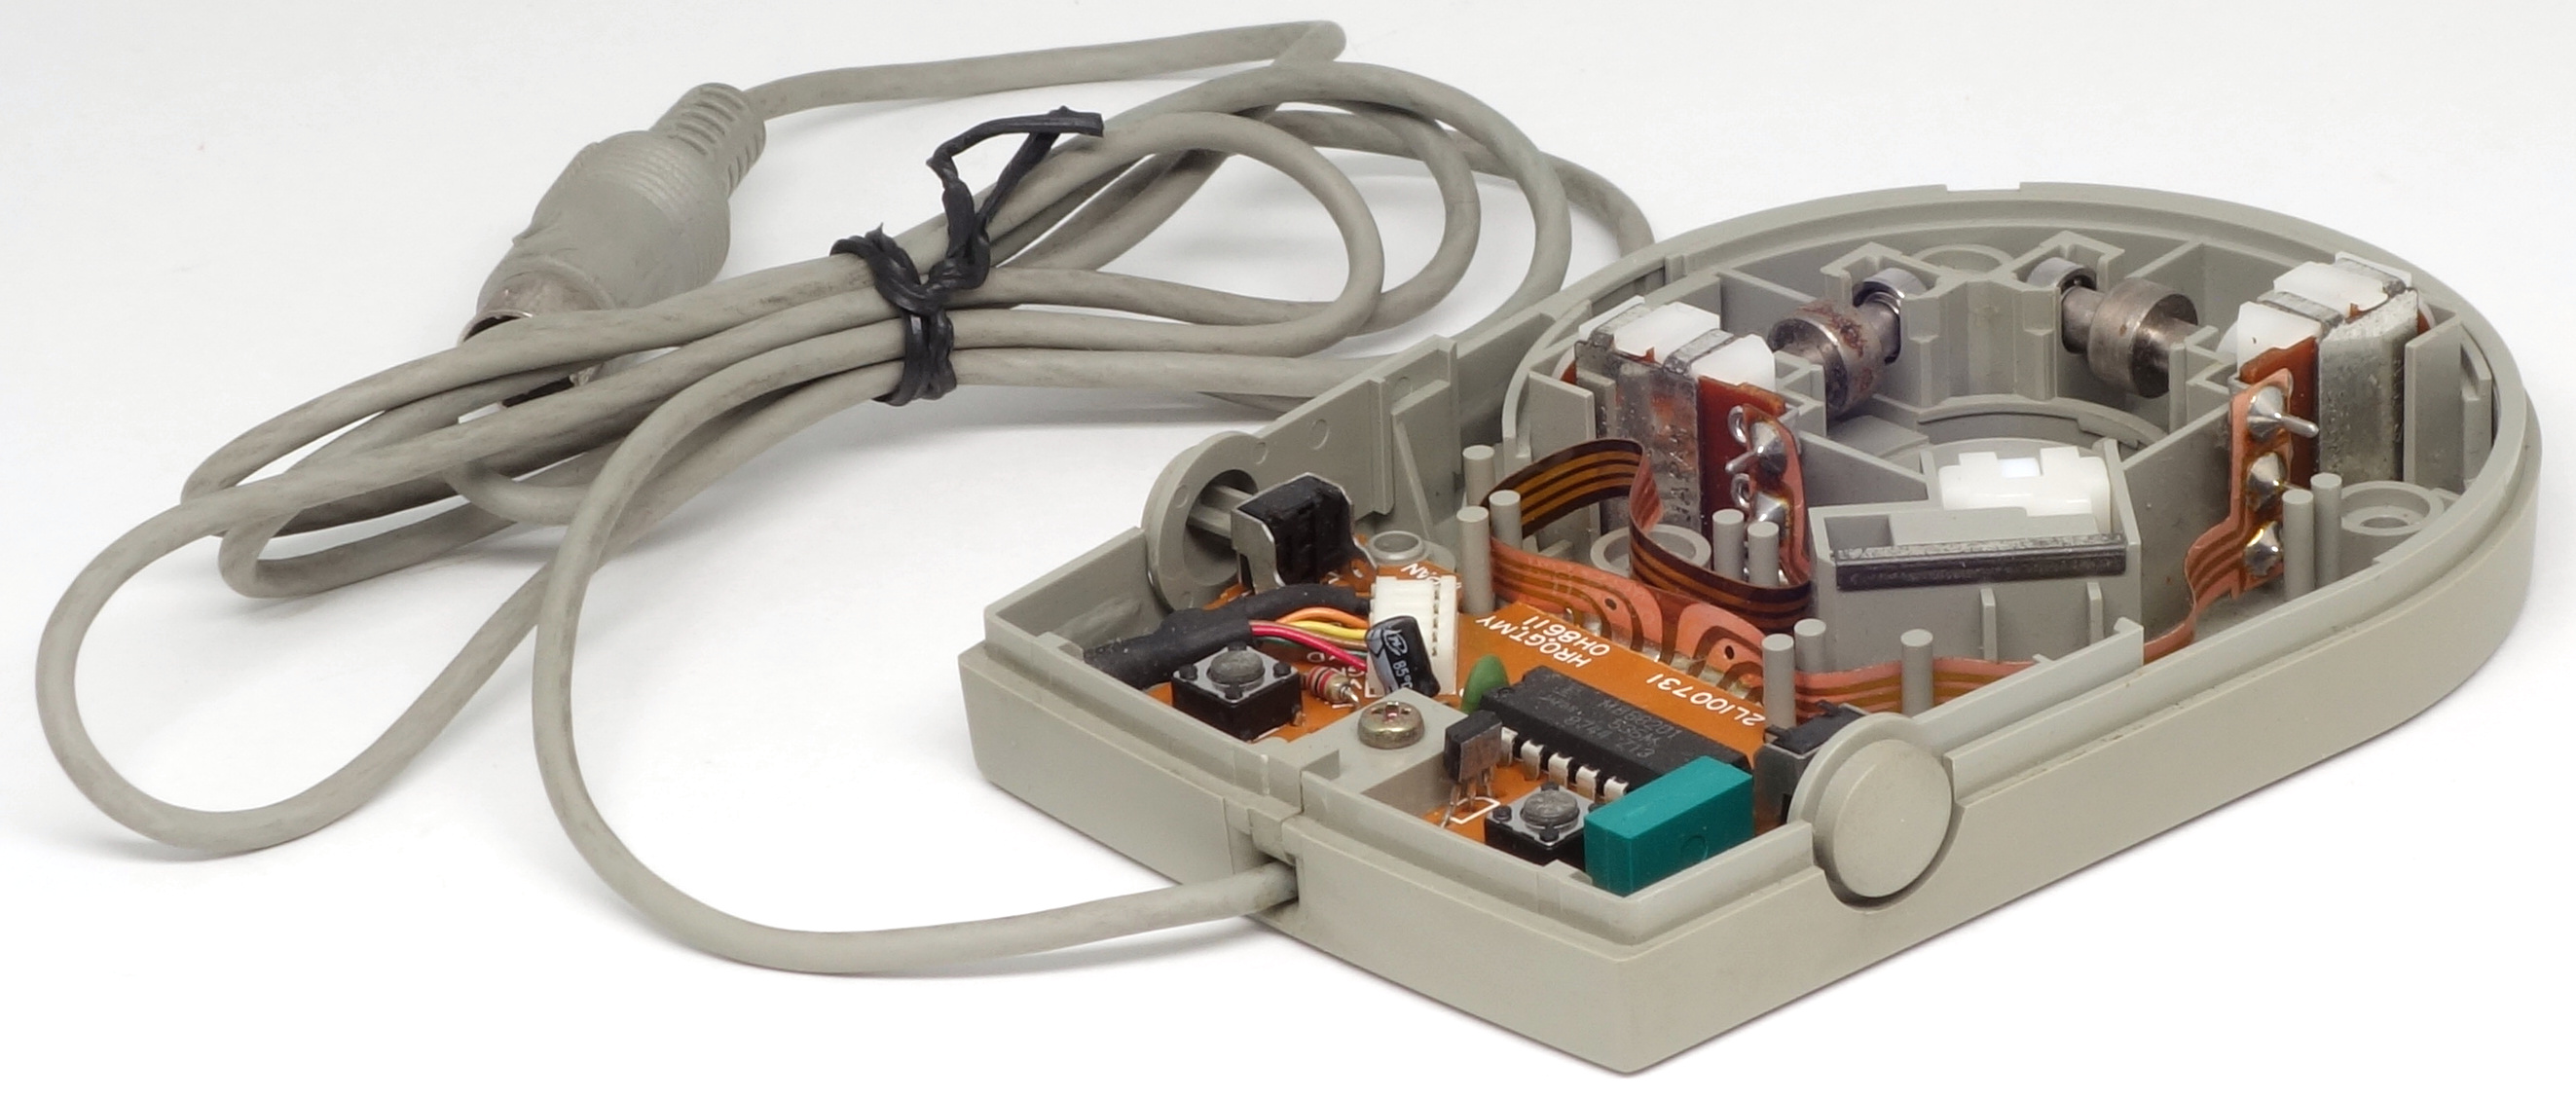
\includegraphics[scale=0.7]{1987_sharp_convertible/inside_30.jpg}
    \caption{Sharp KI-OM0002CE01 disassembled}
    \label{fig:SharpConvertibleInside}
\end{figure}

Examination of the disassembled trackball shows that it uses elements typical of early Alps devices: enclosed mechanical encoders and metal rollers with rolling bearings. In addition to the rotating block, a modification of the standard Alps design is the absence (due to the trackball mode) of a solid plastic structure covering the ball, typical of mice of the 80s and eliminated in later models (fig. \ref{fig:SharpConvertibleInside}). It is also worth noting the funnel-shaped hole in the body, which protects the wire from damage (later computer mice used a ribbed protective sleeve for this purpose).

\begin{thebibliography}{9}
\bibitem {museum} X680000-Computer Museum \url{https://museum.ipsj.or.jp/en/computer/personal/0038.html}
\bibitem{JapaneseVintage} Sharp X86000 Expert -- Japanese Vintage Computer Collection. FEB 2, 2020 \url{https://monochromeeffect.org/JVCC/2020/02/02/x68000-expert/}
\bibitem{JapaneseClickSense} Otonashi. X68000 Z review [in Japanese] - GAME Watch, May 29, 2023 \url{https://game.watch.impress.co.jp/docs/review/rev1/1501505.html}
\end{thebibliography}
\end{document}
